% $Header: /cvsroot/latex-beamer/latex-beamer/examples/beamerexample5.tex,v 1.22 2004/10/08 14:02:33 tantau Exp $

\documentclass[11pt]{beamer}

\usetheme{Darmstadt}

\usepackage{times}
\usefonttheme{structurebold}

%\usepackage[english]{babel}
\usepackage[portuges]{babel}
\usepackage{pgf,pgfarrows,pgfnodes,pgfautomata,pgfheaps}
\usepackage{amsmath,amssymb}
%\usepackage[latin8]{inputenc}
\usepackage[utf8]{inputenc}
\usepackage{graphicx}

\setbeamercovered{dynamic}

\newcommand{\Lang}[1]{\operatorname{\text{\textsc{#1}}}}

\newcommand{\Class}[1]{\operatorname{\mathchoice
  {\text{\sf \small #1}}
  {\text{\sf \small #1}}
  {\text{\sf #1}}
  {\text{\sf #1}}}}

\newcommand{\NumSAT}      {\text{\small\#SAT}}
\newcommand{\NumA}        {\#_{\!A}}

\newcommand{\barA}        {\,\bar{\!A}}

\newcommand{\Nat}{\mathbb{N}}
\newcommand{\Set}[1]{\{#1\}}

\pgfdeclaremask{tu}{beamer-tu-logo-mask}
\pgfdeclaremask{computer}{beamer-computer-mask}
\pgfdeclareimage[interpolate=true,mask=computer,height=2cm]{computerimage}{beamer-computer}
\pgfdeclareimage[interpolate=true,mask=computer,height=2cm]{computerworkingimage}{beamer-computerred}
\pgfdeclareimage[mask=tu,height=.5cm]{logo}{logounesp}

\logo{\pgfuseimage{logo}}

\title{Dualidade Onda-partícula}
\author{Ney Lemke}
\institute[IBB-UNESP]{%
    Mec\^anica Qu\^antica}
\date{2011}                                

\colorlet{redshaded}{red!25!bg}
\colorlet{shaded}{black!25!bg}
\colorlet{shadedshaded}{black!10!bg}
\colorlet{blackshaded}{black!40!bg}

\colorlet{darkred}{red!80!black}
\colorlet{darkblue}{blue!80!black}
\colorlet{darkgreen}{green!80!black}

\def\radius{0.96cm}
\def\innerradius{0.85cm}

\def\softness{0.4}
\definecolor{softred}{rgb}{1,\softness,\softness}
\definecolor{softgreen}{rgb}{\softness,1,\softness}
\definecolor{softblue}{rgb}{\softness,\softness,1}

\definecolor{softrg}{rgb}{1,1,\softness}
\definecolor{softrb}{rgb}{1,\softness,1}
\definecolor{softgb}{rgb}{\softness,1,1}

\newcommand{\Bandshaded}[2]{
  \color{shadedshaded}
  \pgfmoveto{\pgfxy(-0.5,0)}
  \pgflineto{\pgfxy(-0.6,0.1)}
  \pgflineto{\pgfxy(-0.4,0.2)}
  \pgflineto{\pgfxy(-0.6,0.3)}
  \pgflineto{\pgfxy(-0.4,0.4)}
  \pgflineto{\pgfxy(-0.5,0.5)}
  \pgflineto{\pgfxy(4,0.5)}
  \pgflineto{\pgfxy(4.1,0.4)}
  \pgflineto{\pgfxy(3.9,0.3)}
  \pgflineto{\pgfxy(4.1,0.2)}
  \pgflineto{\pgfxy(3.9,0.1)}
  \pgflineto{\pgfxy(4,0)}
  \pgfclosepath
  \pgffill

  \color{black}  
  \pgfputat{\pgfxy(0,0.7)}{\pgfbox[left,base]{#1}}
  \pgfputat{\pgfxy(0,-0.1)}{\pgfbox[left,top]{#2}}
}

\newcommand{\Band}[2]{
  \color{shaded}
  \pgfmoveto{\pgfxy(-0.5,0)}
  \pgflineto{\pgfxy(-0.6,0.1)}
  \pgflineto{\pgfxy(-0.4,0.2)}
  \pgflineto{\pgfxy(-0.6,0.3)}
  \pgflineto{\pgfxy(-0.4,0.4)}
  \pgflineto{\pgfxy(-0.5,0.5)}
  \pgflineto{\pgfxy(4,0.5)}
  \pgflineto{\pgfxy(4.1,0.4)}
  \pgflineto{\pgfxy(3.9,0.3)}
  \pgflineto{\pgfxy(4.1,0.2)}
  \pgflineto{\pgfxy(3.9,0.1)}
  \pgflineto{\pgfxy(4,0)}
  \pgfclosepath
  \pgffill

  \color{black}  
  \pgfputat{\pgfxy(0,0.7)}{\pgfbox[left,base]{#1}}
  \pgfputat{\pgfxy(0,-0.1)}{\pgfbox[left,top]{#2}}
}

\newcommand{\BaenderNormal}
{%
  \pgfsetlinewidth{0.4pt}
  \color{black}
  \pgfputat{\pgfxy(0,5)}{\Band{input tapes}{}}
  \pgfputat{\pgfxy(0.35,4.6)}{\pgfbox[center,base]{$\vdots$}}
  \pgfputat{\pgfxy(0,4)}{\Band{}{}}

  \pgfxyline(0,5)(0,5.5)
  \pgfxyline(1.2,5)(1.2,5.5)
  \pgfputat{\pgfxy(0.25,5.25)}{\pgfbox[left,center]{$w_1$}}

  \pgfxyline(0,4)(0,4.5)
  \pgfxyline(1.8,4)(1.8,4.5)        
  \pgfputat{\pgfxy(0.25,4.25)}{\pgfbox[left,center]{$w_n$}}
  \ignorespaces}

\newcommand{\BaenderZweiNormal}
{%
  \pgfsetlinewidth{0.4pt}
  \color{black}
  \pgfputat{\pgfxy(0,5)}{\Band{Zwei Eingabeb\~AƒÂƒ\~A‚¤nder}{}}
  \pgfputat{\pgfxy(0,4.25)}{\Band{}{}}

  \pgfxyline(0,5)(0,5.5)
  \pgfxyline(1.2,5)(1.2,5.5)
  \pgfputat{\pgfxy(0.25,5.25)}{\pgfbox[left,center]{$u$}}

  \pgfxyline(0,4.25)(0,4.75)
  \pgfxyline(1.8,4.25)(1.8,4.75)        
  \pgfputat{\pgfxy(0.25,4.5)}{\pgfbox[left,center]{$v$}}
  \ignorespaces}

\newcommand{\BaenderHell}
{%
  \pgfsetlinewidth{0.4pt}
  \color{black}
  \pgfputat{\pgfxy(0,5)}{\Bandshaded{input tapes}{}}
  \color{shaded}
  \pgfputat{\pgfxy(0.35,4.6)}{\pgfbox[center,base]{$\vdots$}}
  \pgfputat{\pgfxy(0,4)}{\Bandshaded{}{}}

  \color{blackshaded}
  \pgfxyline(0,5)(0,5.5)
  \pgfxyline(1.2,5)(1.2,5.5)
  \pgfputat{\pgfxy(0.25,5.25)}{\pgfbox[left,center]{$w_1$}}

  \pgfxyline(0,4)(0,4.5)
  \pgfxyline(1.8,4)(1.8,4.5)        
  \pgfputat{\pgfxy(0.25,4.25)}{\pgfbox[left,center]{$w_n$}}
  \ignorespaces}

\newcommand{\BaenderZweiHell}
{%
  \pgfsetlinewidth{0.4pt}
  \color{black}
  \pgfputat{\pgfxy(0,5)}{\Bandshaded{Zwei Eingabeb\~AƒÂƒ\~A‚¤nder}{}}%
  \color{blackshaded}
  \pgfputat{\pgfxy(0,4.25)}{\Bandshaded{}{}}
  \pgfputat{\pgfxy(0.25,4.5)}{\pgfbox[left,center]{$v$}}
  \pgfputat{\pgfxy(0.25,5.25)}{\pgfbox[left,center]{$u$}}%

  \pgfxyline(0,5)(0,5.5)
  \pgfxyline(1.2,5)(1.2,5.5)

  \pgfxyline(0,4.25)(0,4.75)
  \pgfxyline(1.8,4.25)(1.8,4.75)        
  \ignorespaces}

\newcommand{\Slot}[1]{%
  \begin{pgftranslate}{\pgfpoint{#1}{0pt}}%
    \pgfsetlinewidth{0.6pt}%
    \color{structure}%
    \pgfmoveto{\pgfxy(-0.1,5.5)}%
    \pgfbezier{\pgfxy(-0.1,5.55)}{\pgfxy(-0.05,5.6)}{\pgfxy(0,5.6)}%
    \pgfbezier{\pgfxy(0.05,5.6)}{\pgfxy(0.1,5.55)}{\pgfxy(0.1,5.5)}%
    \pgflineto{\pgfxy(0.1,4.0)}%
    \pgfbezier{\pgfxy(0.1,3.95)}{\pgfxy(0.05,3.9)}{\pgfxy(0,3.9)}%
    \pgfbezier{\pgfxy(-0.05,3.9)}{\pgfxy(-0.1,3.95)}{\pgfxy(-0.1,4.0)}%
    \pgfclosepath%
    \pgfstroke%
  \end{pgftranslate}\ignorespaces}

\newcommand{\SlotZwei}[1]{%
  \begin{pgftranslate}{\pgfpoint{#1}{0pt}}%
    \pgfsetlinewidth{0.6pt}%
    \color{structure}%
    \pgfmoveto{\pgfxy(-0.1,5.5)}%
    \pgfbezier{\pgfxy(-0.1,5.55)}{\pgfxy(-0.05,5.6)}{\pgfxy(0,5.6)}%
    \pgfbezier{\pgfxy(0.05,5.6)}{\pgfxy(0.1,5.55)}{\pgfxy(0.1,5.5)}%
    \pgflineto{\pgfxy(0.1,4.25)}%
    \pgfbezier{\pgfxy(0.1,4.25)}{\pgfxy(0.05,4.15)}{\pgfxy(0,4.15)}%
    \pgfbezier{\pgfxy(-0.05,4.15)}{\pgfxy(-0.1,4.2)}{\pgfxy(-0.1,4.25)}%
    \pgfclosepath%
    \pgfstroke%
  \end{pgftranslate}\ignorespaces}

\newcommand{\ClipSlot}[1]{%
  \pgfrect[clip]{\pgfrelative{\pgfxy(-0.1,0)}{\pgfpoint{#1}{4cm}}}{\pgfxy(0.2,1.5)}\ignorespaces}

\newcommand{\ClipSlotZwei}[1]{%
  \pgfrect[clip]{\pgfrelative{\pgfxy(-0.1,0)}{\pgfpoint{#1}{4.25cm}}}{\pgfxy(0.2,1.25)}\ignorespaces}


\AtBeginSection[]{\frame{\frametitle{Outline}\tableofcontents[current]}}

\begin{document}

\frame{\titlepage}

%\section*{Outline}

\frame{\frametitle{Outline}\tableofcontents} 

\section{Prolegômeno}
\frame{\frametitle{Base Experimental}
  \begin{itemize}
  \item Fótons são partículas e ondas: $E=h\nu=\hbar\omega$
  \item Elétrons são partículas e ondas: $p=\frac{h}{ \lambda}=\hbar k$
  \end{itemize}
}


\section{Pacotes de Onda}

\frame{\frametitle{Pacote de Onda}
$$\psi (x,t)=A e^{i(kx-\omega t)}$$

onde $\omega=2\pi\nu$ é a frequência angular e $k=2 \pi/\lambda$ é o
número de onda.  }


\frame{\frametitle{Onda de Luz}

  No caso de uma onda de luz no vácuo, temos que:
$$\nu=\frac{c}{\lambda}$$
$$\omega=c k$$
em um meio dispersivo temos o caso mais geral:

$$\omega=\omega(k)$$

Em linhas gerais isso significa que luz se propaga com uma velocidade
que depende do comprimeto de onda.  } 

\frame{\frametitle{Pacote de Onda} 
Como transformar um onda em partícula?

A solução de Schrödinger é somar um número muito grande de ondas 
para obter uma distribuição concentrada.

$$\psi(x,t)=\int_{-\infty}^\infty A(k) e^{i (kx - \omega t)}$$

Intuitivamente podemos pensar que:

$$\lim_{L->\infty} \sum_{n=-\infty}^\infty A_n \exp \left( \frac{i n \pi x}{L}\right)=\int_{-\infty}^\infty A(k) e^{i (kx - \omega t)}$$

onde $n=k/L$, para facilitar pense que ``a corda'' está em $[-L/2, L/2]$.
}

\frame{\frametitle{Exemplo} 
Considere o caso:

$$A(k)=\exp \left( \frac{-\alpha(k-k_o)^2}{2} \right)$$

Neste caso teremos que:

$$\psi(x,0)=\int_{-\infty}^\infty A \exp \left( \frac{-\alpha (k-k_o)^2}{2} \right) e^{ikx}$$



} 


\frame{\frametitle{Exemplo} 
Para fazer este cálculo vamos usar a integral tabelada (Tabela Schaum 15.75):

$$\int_{-\infty}^\infty e^{-(ax^2+bx+c)}\,dx=\sqrt\frac{\pi}{a}e^{(b^2-4 ac)/4a}$$

Obtemos que:

$$\psi(x,0)=\sqrt{\frac{2 \pi}{\alpha}}e^{ik_o x}e^{-x^2/2 \alpha}$$

} 


\frame{\frametitle{Exemplo} 
\begin{center}
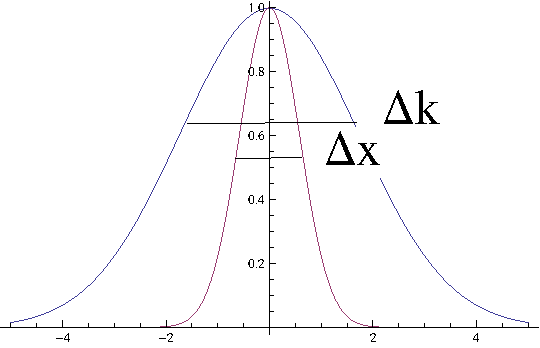
\includegraphics[scale=0.5]{pacotes}
\end{center}

Considerando 

$$e^{-x_L^2/2 \alpha}\sim e^{-1/2}$$

$$\Delta x=2|x_L|$$

Procedendo de forma análoga para $k$ podemos concluir que:

$$\Delta x\Delta k\sim 4$$

Este resultado é importante por que ilustra o fato de que para construir
pacotes cocentrados em $x$ precisamos somar ondas de muitos comprimentos
de onda. 

} 



\frame{\frametitle{Movimento do Pacote} 
No caso mais geral $\omega=\omega(k)$, vamos caracterizar esse movimento.

$$\omega (k)=\omega(k_o)
+(k-k_o)\left( \frac{\partial \omega}{\partial k} \right)_{k=k_o}
+(k-k_o)^2\left( \frac{\partial^2 \omega}{\partial k^2} \right)_{k=k_o}
$$


\begin{eqnarray*}
kx -\omega t&=&(k_o x-\omega(k_o)t) \\
&+& (k-k_o)\left[ x-\left( \frac{\partial \omega}{\partial k} \right)_{k=k_o}t \right]\\
&+& (k-k_o)^2\left( \frac{\partial^2 \omega}{\partial k^2} \right)_{k=k_o}t
\end{eqnarray*}
}

\frame{\frametitle{Movimento do Pacote} 
Definimos a velocidade de grupo por:

$$v_g=\left( \frac{\partial \omega}{\partial k} \right)_{k=k_o}$$

Esta velocidade estará associada ao movimento do pacote como um todo. 
}

\frame{\frametitle{Movimento do Pacote} 
$$\psi(x,t)=\int_{-\infty}^\infty dk A(k) e^{i (kx - \omega t)}$$

Definindo $q=k-k_o$ e 

$$\beta=\left( \frac{\partial^2 \omega}{\partial k^2} \right)_{k=k_o}$$

temos que:

$$\psi(x,t)=e^{i(k_o-\omega(k_o)t)}\int_{-\infty}^\infty\, dq A(q+k_o)e^{iq(x-v_g t)}e^{-i\frac{q^2}{2}\beta t}
$$

} 


\frame{\frametitle{Caso Particular} 
Considere agora:

$$A(q+k_o)=e^{-\alpha q^2/2}$$
\begin{eqnarray*}
\psi(x,t)&=&e^{i(k_o-\omega(k_o)t)}\int_{-\infty}^\infty\, dq e^{-\alpha q^2/2} e^{iq(x-v_g t)}e^{-i\frac{q^2}{2}\beta t}\\
&=& \sqrt{\frac{2 \pi}{\alpha+2 i \beta t}}e^{i(k_o x-\omega(k_o)) t}e^{\frac{-(x-v_g t)^2}{2 \alpha +4 i \beta t}}
\end{eqnarray*}


\begin{eqnarray*}
|\psi(x,t)|^2&=&\psi(x,t)\psi^*(x,t)\\
&=& \frac{2 \pi}{\sqrt{\alpha^2 + 4\beta^2 t^2}}e^{\frac{-(x-v_gt)^2}{\alpha^2+ 4 \beta^2 t^2}}
\end{eqnarray*}
}

\frame{\frametitle{Pacote de Onda} 

\begin{center}
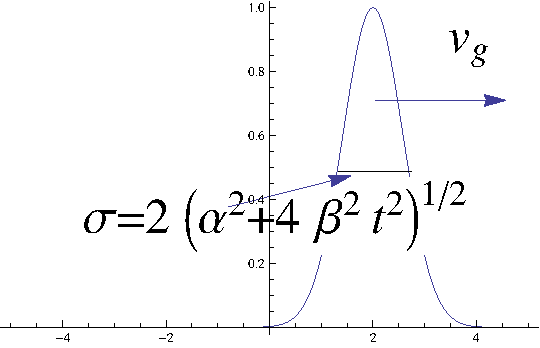
\includegraphics[scale=0.5]{pacmov}
\end{center}
}


\frame{\frametitle{Interpretação Probabilística} 
$$P(x,t)dx=|\psi(x,t)|^2 dx$$

O módulo quadrado  da função de onda está relacionado a probabilidade 
de encontramos a partícula em algum ponto. 

Note que a função de onda que representa uma partícula deve ser complexa para
conseguirmos representar o fenômeno de interferência. 

Seja $\psi=\psi_1+\psi_2$ temos que:

\begin{eqnarray*}
  |\psi|^2&=&(\psi_1+\psi_2)(\psi_1^* +\psi_2^*)\\
&=&|\psi_1|^2+|\psi_2|^2+2\Re(\psi_1\psi_2^*)
\end{eqnarray*}

}


\frame{\frametitle{Plano}
  \begin{itemize}
  \item Partículas são descritas por somatórios de ondas.
  \item A velocidade clássica equivale a velocidade de grupo.
  \item A dispersão do pacote está relacionado ao erro da medida.
  \end{itemize}


}
\section{Equação de Schrödinger}

\frame{\frametitle{Relações de Broglie} 
$$k=\frac{p}{\hbar}$$

$$\omega=\frac{E}{\hbar}$$

$$\psi(x,t)=\frac{1}{\sqrt{2\pi \hbar}}\int_{-\infty}^\infty dp \phi(p) e^{i(p x- Et)/\hbar}$$

}

\frame{\frametitle{Partícula Livre} 
$$v_g=\frac{\partial \omega}{\partial k}=\frac{\partial E}{\partial p}=\frac{p}{m}$$

$$E=\frac{p^2}{2 m}$$


}

\frame{\frametitle{Teorema PL} 

$$i\hbar\frac{\partial \psi(x,t)}{\partial t}=\frac{-\hbar^2}{2 m}\frac{\partial^2 \psi (x,t)}{\partial x^2}$$

Basta usar a definição:

$$
\psi(x,t)=\frac{1}{\sqrt{2\pi \hbar}}\int_{-\infty}^\infty dp \phi(p) e^{i(px-Et)/\hbar}
$$



}

\frame{\frametitle{Equação de Schrödinger} 

No caso geral temos que:

$$E=\frac{p^2}{2 m}+V(x)$$

$$i\hbar\frac{\partial \psi(x,t)}{\partial t}=\left[ \frac{-\hbar^2}{2 m}\frac{\partial^2}{\partial x^2} +V(x)\right] \psi(x,t)$$
}

\frame{\frametitle{Função de onda no espaço $p$} 
$$\psi(x,0)=\frac{1}{\sqrt{2\pi \hbar}}\int_{-\infty}^\infty dp \phi(p) e^{ipx/\hbar}$$

$\phi(p)$=?


\begin{eqnarray*}
\int_{-\infty}^\infty \psi(x,0)e^{-ip^\prime x/\hbar}\,dx&=&
\frac{1}{\sqrt{2\pi\hbar}}\int_{-\infty}^\infty\int_{-\infty}^\infty dpdx
\phi(p)e^{ix(p-p^\prime)/\hbar} \\
&=&\frac{1}{\sqrt{2\pi \hbar}}
\int_{-\infty}^\infty dp \phi(p) 2 \pi \hbar
\delta(p-p^\prime) \\
&=& \sqrt{2\pi\hbar}\phi(p^\prime)
\end{eqnarray*}

$$\phi(p)=\frac{1}{\sqrt{2\pi \hbar}}\int_{-\infty}^\infty dx e^{-ip x/\hbar}\psi(x,0)\,dx$$
}

\frame{\frametitle{Integral} 


$$\int_{-\infty}^\infty e^{i p x/\hbar}\, dx=
\lim_{\epsilon\to 0} \int_{-\infty}^\infty dx e^{ipx/\hbar -\epsilon |x|}$$

Sabemos que 

$$\int_{-\infty}^\infty dp \delta(p)=1$$

Calculando esta integral para o nosso caso:

$$\lim_{\epsilon\to 0} \int_{-\infty}^\infty dx \int_{-\infty}^\infty dp e^{ipx/\hbar -\epsilon |x|}=$$

$$\lim_{\epsilon\to 0} \int_{-\infty}^\infty dx \int_{-\infty}^\infty dp \cos(p x/\hbar) e^{-\epsilon |x|}=$$


}

\frame{\frametitle{Integral} 
$$\lim_{\epsilon\to 0} \int_{-\infty}^\infty dp \frac{2 \hbar^2\epsilon}{p^2+\hbar^2\epsilon^2}=$$

$$\lim_{\epsilon\to 0} 2 \pi\hbar=2 \pi\hbar$$

Logo temos que:

$$\int_{-\infty}^\infty e^{i p x/\hbar}\, dx=2\pi \hbar\delta (p)$$
}


\section{Interpretação}

\frame{\frametitle{Relações de Incerteza de Heisenberg} 

$$\Delta x\Delta p\geq \frac{\hbar}{2}$$

Para construir um pacote de onda temos que somar ondas com vários ``comprimentos'' de onda, isso equivale a somar ondas com diferentes ``velocidades''  de
propagação. Ou seja para concentrar a partícula em uma posição vamos precisar
de uma distribuição larga nos momentos. 
}


\frame{\frametitle{Órbitas de Bohr} 
Para observar uma órbita de Bohr precisariamos de um fóton com comprimento de onda pequeno em comparação com a diferença entre as órbitas.

$$\lambda << r_{n+1}-r_n$$
$$<< \frac{\hbar}{m c \alpha}[(n+1)^2-n^2]\sim \frac{\hbar n}{m c \alpha}$$
$$p_\gamma=\frac{\hbar}{\lambda}>>\frac{mc\alpha}{n}$$

$$\Delta E=\frac{p\Delta p}{m}\sim \frac{pp_\gamma}{m}>>\frac{m(c\alpha)^2}{n^2}$$
Compare com as energias de Bohr:

$$E=\frac{m (\alpha c)^2}{n^2}$$
}

\frame{\frametitle{Princípio da Incerteza para a Energia} 
$$\Delta E \Delta t \geq \hbar$$

Esta equação é mais difícil de interpretar que a anterior. Mas de qualquer forma
ela possui aplicações em Físicas de partículas relacionando a incerteza da massa
com a meia vida. 
}



\frame{\frametitle{Comentários} 
\begin{center}
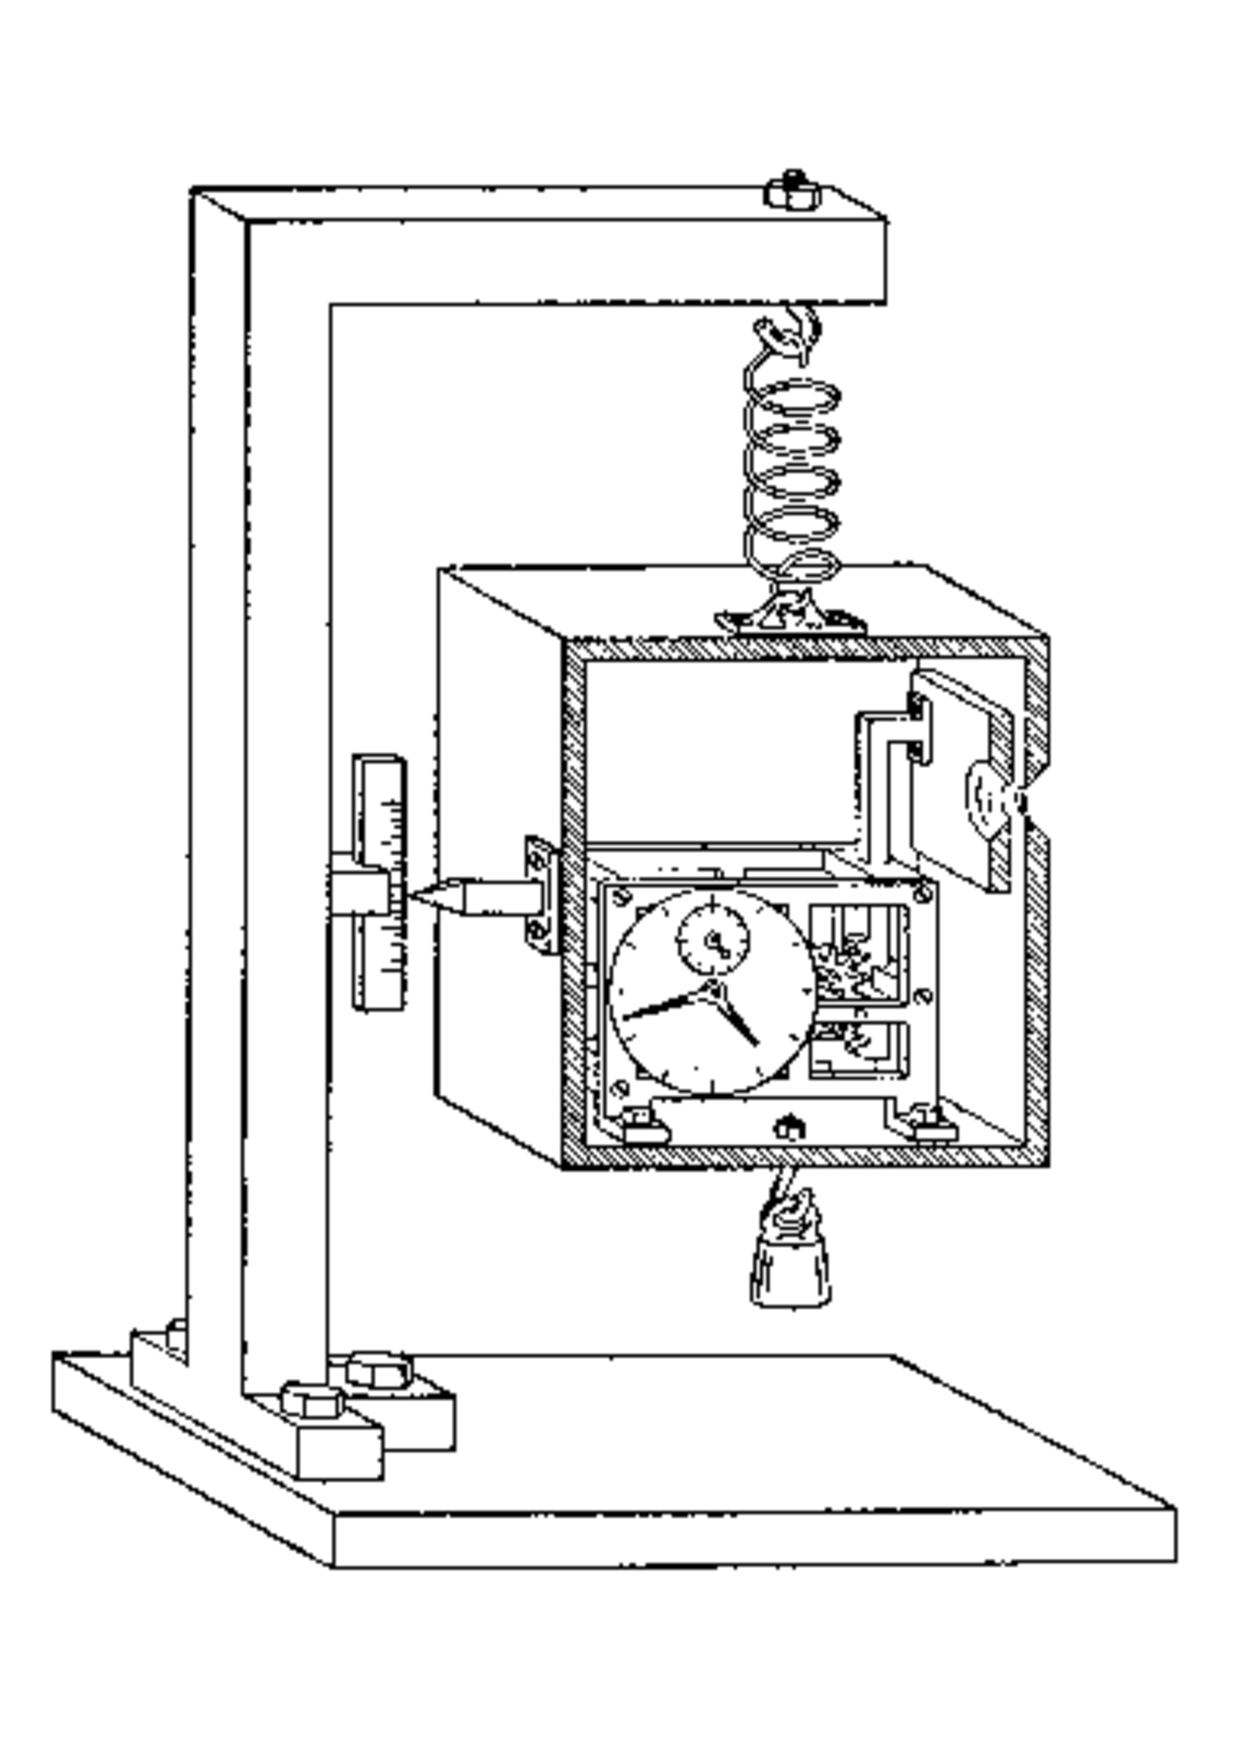
\includegraphics[scale=0.25]{bohrarg}
\end{center}
}

\frame{\frametitle{Comentários} 
  \begin{itemize}
  \item O princípio da Incerteza não é um princípio, ele é 
uma consequência da MQ.
\item Ele não afirma que as teorias não possam fazer predições com precisão 
absoluta. Ex. podemos medir a posição  com precisão arbitrária. 
\item O que não podemos fazer é que as partículas possuem simultaneamente 
posição e momento bem definidos. 
  \end{itemize}
}

\frame{\frametitle{Comentários} 
\begin{center}
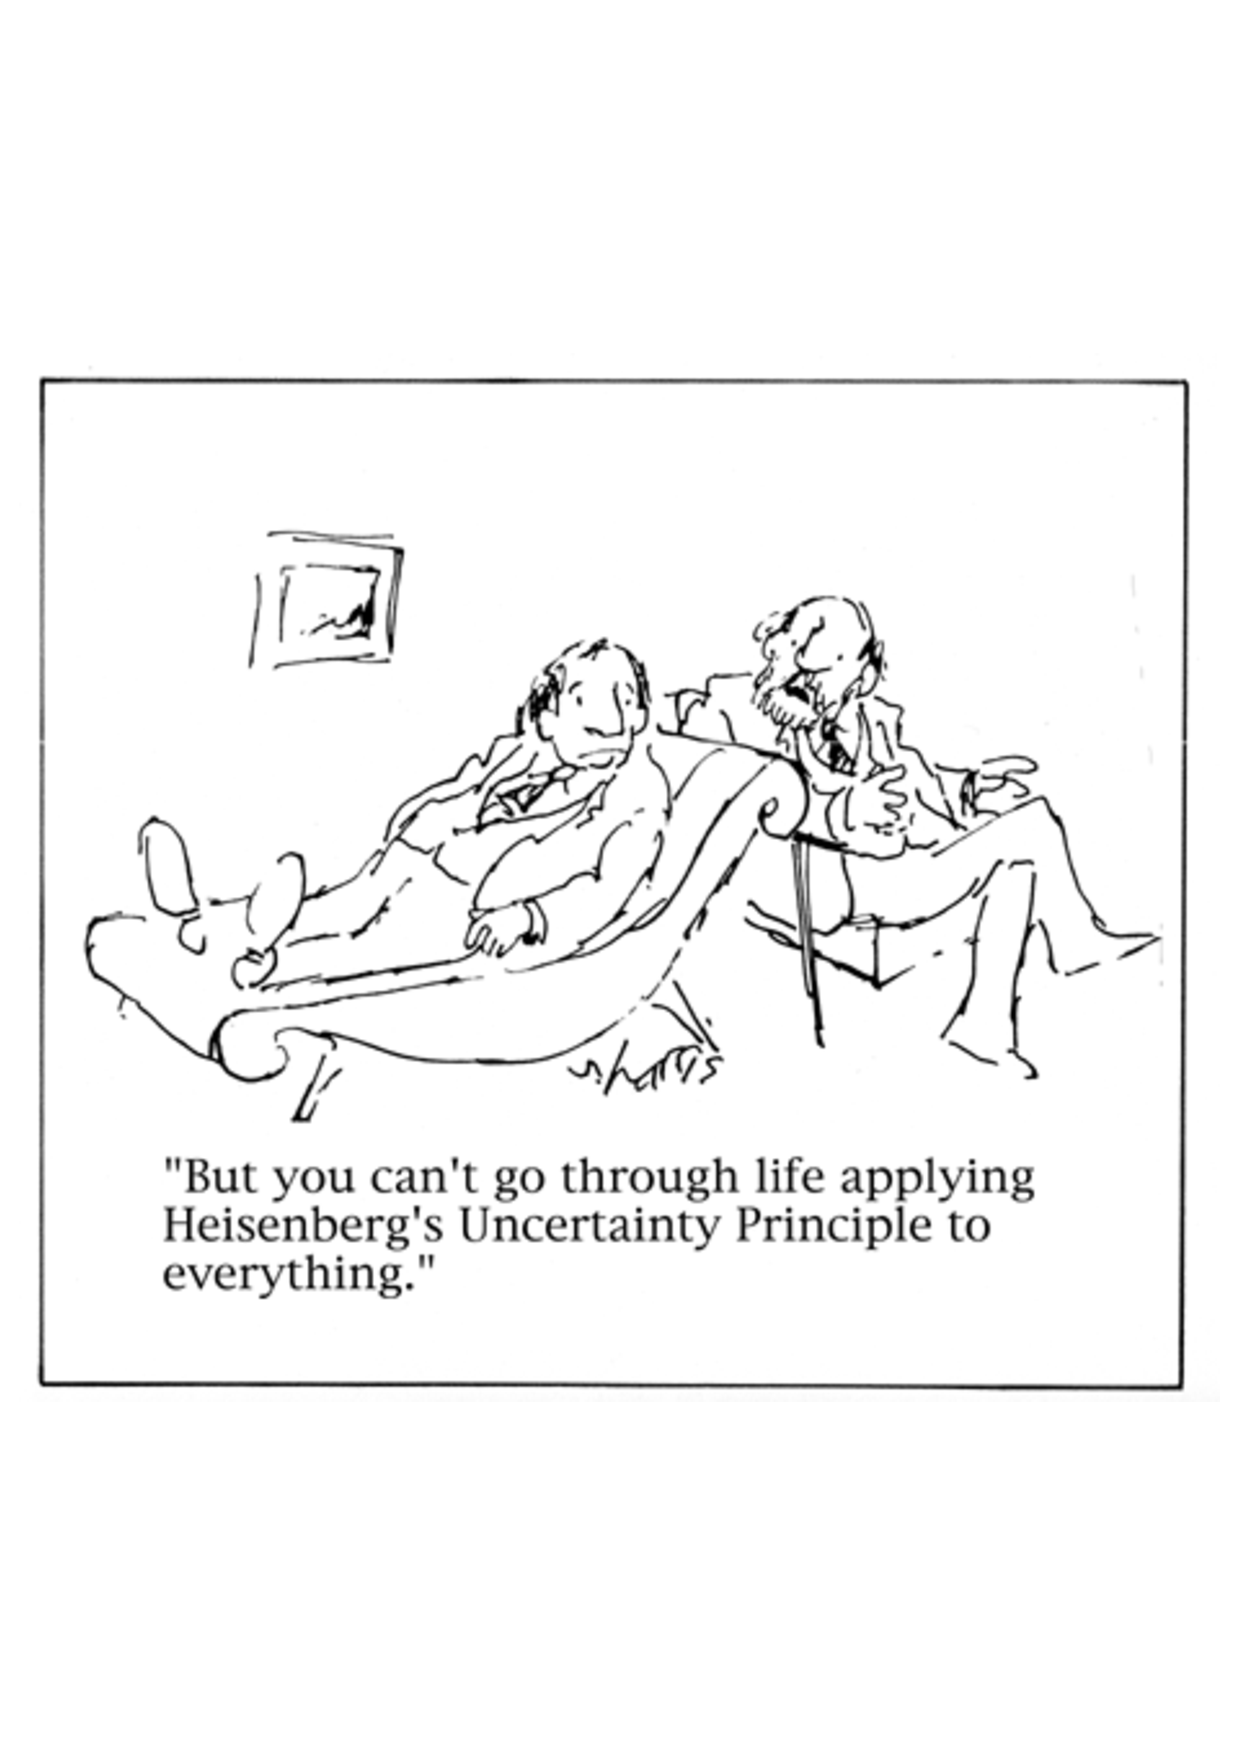
\includegraphics[scale=0.3]{incerteza}
\end{center}
}


\frame{\frametitle{Interpretação Probalística}
$$\int_{-\infty}^\infty P(x,t)\, dx=\int_{-\infty}^\infty |\psi (x,t)|^2 \, dx=1$$

$$\int_{-\infty}^\infty \psi^* (x,t)x^n\psi(x,t)  \, dx<\infty$$

$$\int_{-\infty}^\infty \psi^* (x,t)\frac{\partial^n}{\partial x^n}\psi(x,t)  \, dx<\infty$$
}

\frame{\frametitle{Corrente de Probabilidade}

$$-i \hbar \frac{\partial \psi^*}{\partial t}= -\frac{\hbar^2}{2m} \frac{\partial^2\psi^*}{\partial x^2}+V(x)\psi^*$$

$$\frac{\partial P(x,t)}{\partial t}=\psi\frac{\partial\psi^*}{\partial t}+
\psi^*\frac{\partial\psi}{\partial t}$$

$$=\frac{1}{i\hbar}\frac{\hbar^2}{2 m}\left( \psi\frac{\partial^2 \psi^*}{\partial x^2}-\psi^*\frac{\partial^2 \psi}{\partial x^2}\right)$$

$$=-\frac{\partial}{\partial x}\left[ \frac{\hbar}{2 i m} 
\left(
\psi^*\frac{\partial \psi}{\partial x }-\psi\frac{\partial \psi^*}{\partial x }
\right)\right]
$$

}


\frame{\frametitle{Corrente de Probabilidade}

$$ j(x,t)=\frac{\hbar}{2 i m} 
\left(
\psi^*\frac{\partial \psi}{\partial x }-\psi\frac{\partial \psi^*}{\partial x }
\right)$$

$$\frac{\partial P(x,t)}{\partial t}+\frac{\partial j(x,t)}{\partial x}=0$$

}


\frame{\frametitle{Corrente de Probabilidade}

$$\int_{-\infty}^\infty \,dx \frac{\partial P(x,t)}{\partial t}+
\int_{-\infty}^\infty \,dx \frac{\partial j(x,t)}{\partial x}$$

$$ \frac{\partial }{\partial t}\int_{-\infty}^\infty \,dx P(x,t)+
j(\infty,t)-j(-\infty,t)$$

O primeiro termo é zero pois a integral é sempre 1 e o segundo
é zero porque não existem correntes vindos do infinito. 

}


\frame{\frametitle{Valores Esperados}
$$\langle f(x) \rangle = \int_{-\infty}^\infty f(x) P(x,t) \, dx$$

$$\langle f(x) \rangle = \int_{-\infty}^\infty \psi^*(x,t) f(x) \psi(x,t) \, dx$$
}


\frame{\frametitle{Valores Esperados}


$$p=m \frac{d x}{d t}$$

$$\langle p \rangle = m \frac{d\langle x \rangle}{d t}=m\frac{d}{dt}\int_{-\infty}^\infty dx \psi^*x\psi$$

$$=m \int_{-\infty}^\infty dx \left[ \frac{d\psi^*}{dt} x \psi + \psi^* x\frac{d \psi}{dt} \right]$$

$$=\frac{-m}{i\hbar}  \int_{-\infty}^\infty dx 
\left[
\left(
\frac{-\hbar^2}{2m} \frac{\partial^2 \psi^*}{\partial x^2}+V(x)\psi^*
\right)x\psi
\right.
$$

$$
-\left.
\left(
\frac{-\hbar^2}{2m} \frac{\partial^2 \psi}{\partial x^2}+V(x)\psi
\right)x\psi^*
\right]
$$
}

\frame{\frametitle{Valores Esperados}
$$=\frac{-m}{i\hbar}  \int_{-\infty}^\infty dx 
\left[
\left(
\frac{-\hbar^2}{2m} \frac{\partial^2 \psi^*}{\partial x^2}
\right)x\psi\right.$$

$$
\left.
-
\left(
\frac{-\hbar^2}{2m} \frac{\partial^2 \psi}{\partial x^2}
\right)x\psi^*
\right]
$$

Note que:

$$\psi x\frac{\partial^2 \psi^*}{\partial x^2}-
\psi^* x\frac{\partial^2 \psi}{\partial x^2}=$$

$$
\frac{\partial}{\partial x}\left[
\frac{\psi^*}{\partial x} x \psi 
-\frac{\psi}{\partial x} x \psi^* -\psi\psi^* 
\right]
+2\psi^*\frac{\partial \psi}{\partial x}
$$

$$\langle p \rangle = \frac{\hbar}{2 i}\int_{-\infty}^\infty dx 
2\psi^*\frac{\partial\psi}{\partial x}$$
}

\frame{\frametitle{Valores Esperados}
$$\langle p \rangle=\int_{-\infty}^\infty dx \psi^* \left( \frac{\hbar}{i} \frac{\partial}{\partial x}  \right)\psi
$$
}

\frame{\frametitle{Valores Esperados}

$$\langle p^n\rangle 
=\int_{-\infty}^\infty dx \psi^* \left( \frac{\hbar}{i} \frac{\partial}{\partial x}  \right)^n\psi
$$

$$\langle f(p) \rangle 
=\int_{-\infty}^\infty dx \psi^* f\left( 
\frac{\hbar}{i} \frac{\partial}{\partial x}  \right)
\psi
$$

$$\hat{p}=\left( \frac{\hbar}{i} \frac{\partial}{\partial x}  \right)$$
}

\frame{\frametitle{Operadores}
$$\hat{H}=\frac{\hat{p}^2}{2 m}+V(x)$$

Equação de Schrödinger

$$i\hbar\frac{\partial \psi}{\partial t}=\hat{H} \psi $$
}

\frame{\frametitle{Funções de onda em $p$}

$$\phi(p)=\frac{1}{\sqrt{2\pi\hbar}}\int_{-\infty}^\infty dx e^{-ip x/\hbar}\psi(x,0)\,dx$$

$$\int_{-\infty}^\infty dp \phi^*(p)\phi(p)=$$
$$ \int_{-\infty}^\infty dp \phi^*(p) \frac{1}{\sqrt{2\pi \hbar}}\int_{-\infty}^\infty\,dx
\psi(x)e^{-ipx/\hbar}= $$

$$
 \frac{1}{\sqrt{2\pi \hbar}}\int_{-\infty}^\infty dx \psi(x)  \int_{-\infty}^\infty\,dp
\phi^*(p) e^{-ipx/\hbar}= 
$$


$$
\int_{-\infty}^\infty dx \psi(x)\psi^*(x)=1 
$$

}


\frame{\frametitle{Funções de onda em $p$}

$$\langle p \rangle =\int_{-\infty}^\infty dx \psi^*(x)
\left(\frac{\hbar}{i}\frac{\partial}{\partial x} 
\right)
\psi(x)$$

$$\langle p \rangle =\frac{1}{\sqrt{2\pi\hbar}}\int_{-\infty}^\infty dx \psi^*(x)
\left(\frac{\hbar}{i}\frac{\partial}{\partial x} 
\right)
\int_{-\infty}^\infty dp\phi(p)e^{ipx/\hbar}
$$

$$\langle p \rangle =\frac{1}{\sqrt{2\pi\hbar}}\int_{-\infty}^\infty dp\phi(p) 
\int_{-\infty}^\infty dx p\psi^* e^{ipx/\hbar}
=\int_{-\infty}^\infty dp\phi^*(p)p\phi(p)
$$
}

\frame{\frametitle{Funções de onda em $p$}
$$\langle x \rangle 
=\int_{-\infty}^\infty dp\phi^*(p)
\left(
i\hbar\frac{\partial }{\partial p}
\right)
\phi(p)
$$
}

\frame{\frametitle{Exemplo}


\begin{tabular}{c c}
   \begin{minipage}{0.45\textwidth}
     \begin{center}
Seja $\psi(x)=2\alpha^{3/2}x e^{-\alpha x}$ se $x>0$ e zero nos demais casos. 

  \begin{itemize}
  \item Determine a posição do máximo de $P(x)$.
  \item Determine $\langle x \rangle$ e $\langle x^2 \rangle$,
  \item Qual é a probabilidade de encontrar a partícula entre $x=0$ e $x=1/\alpha$?
  \item Calcule $\phi(p)$, $\langle p \rangle$ e $\langle p^2 \rangle$,
  \end{itemize}
      
     \end{center}
    \end{minipage}&
    \begin{minipage}{0.45\textwidth} 
 \includegraphics[scale=0.3]{schaum}
  
 \end{minipage}
\end{tabular}


}

\frame{\frametitle{Comutação}


$$x\hat{p}\psi=-i\hbar x\frac{\partial \psi}{\partial x}$$

$$\hat{p}x\psi=-i\hbar \frac{\partial x \psi}{\partial x}=-i\hbar\psi-i\hbar\frac{\partial \psi}{\partial x}$$

$$x\hat{p}-\hat{p}x=[x,\hat{p}]=i\hbar$$
}

\frame{\frametitle{Comentarios} 
\begin{center}
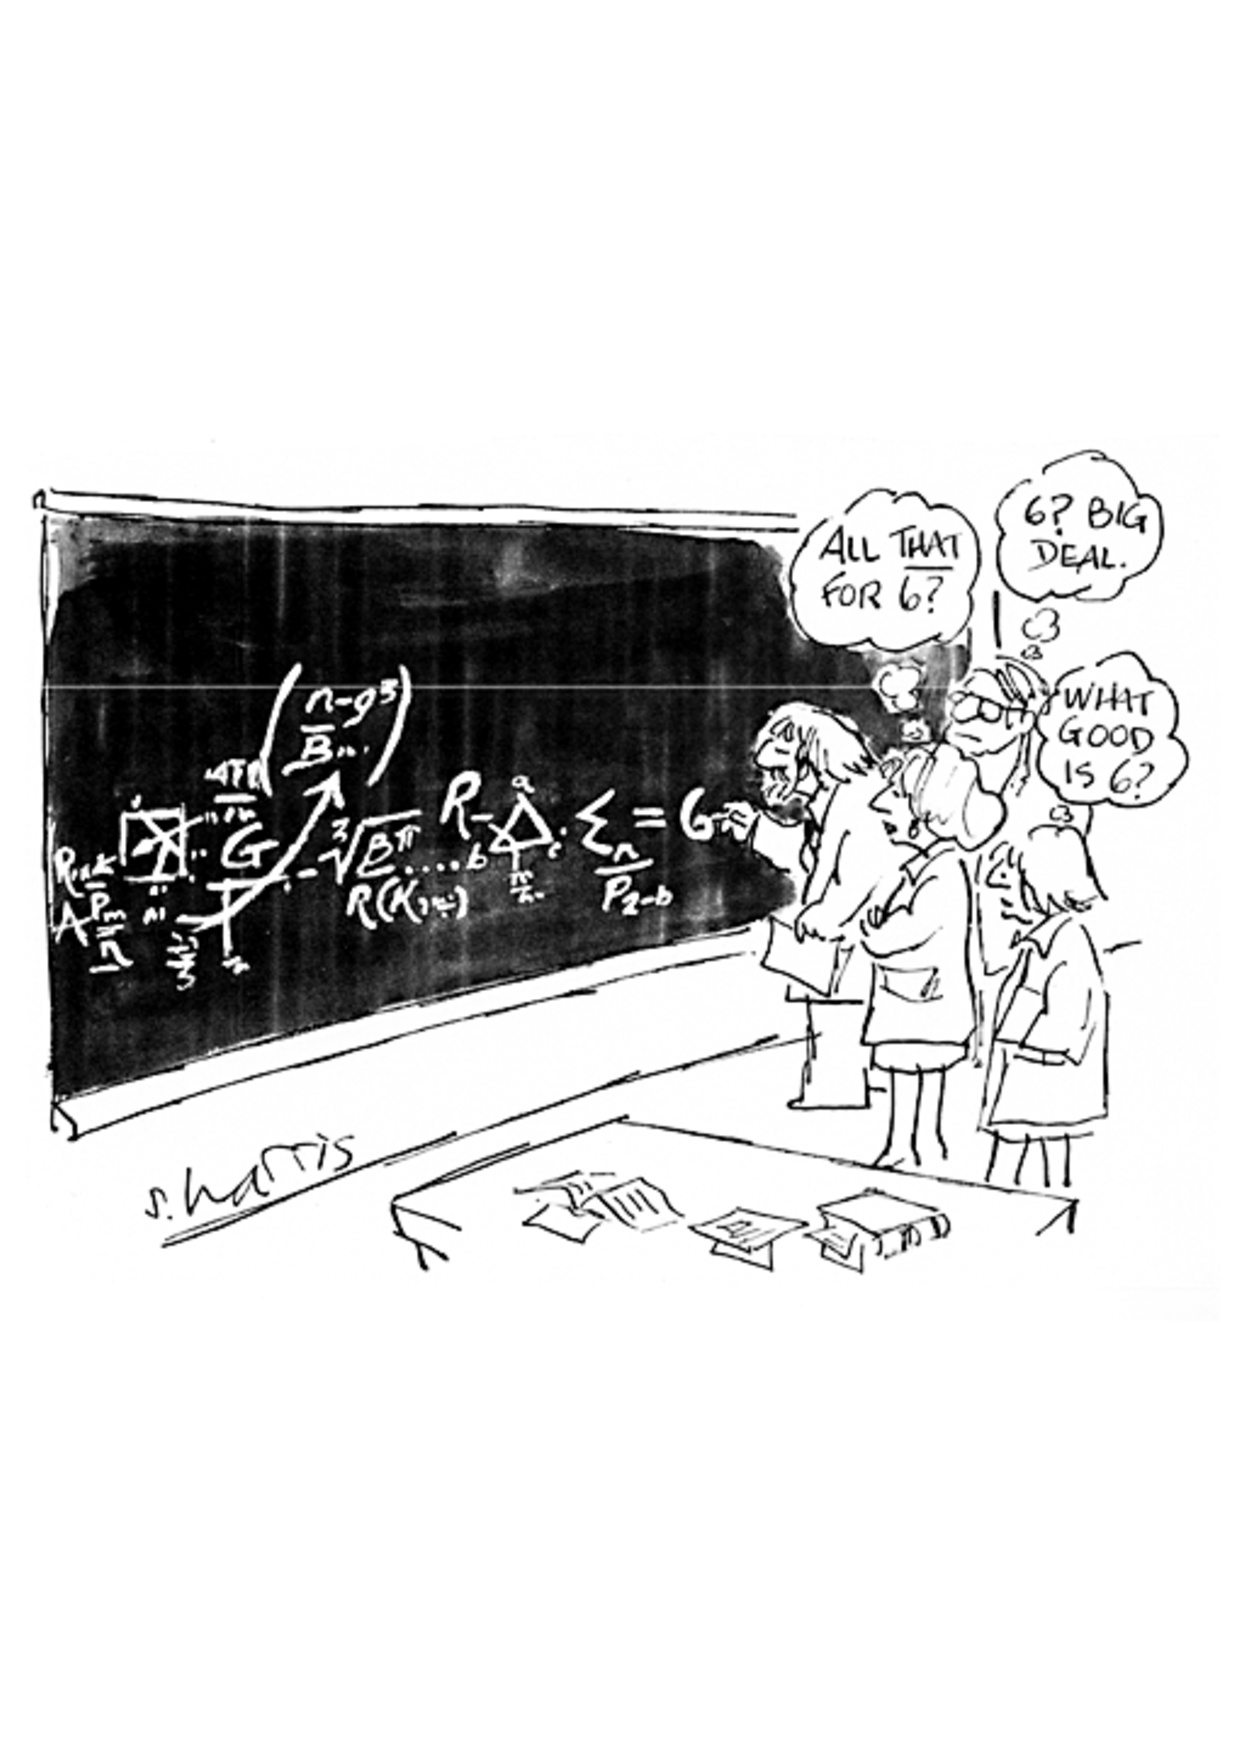
\includegraphics[scale=0.3]{six}
\end{center}
}

\end{document}
